\documentclass[a4paper]{article}
\usepackage[italian]{babel}
\usepackage[left=1cm, right=1cm, bottom=2cm, top=2cm]{geometry}
\usepackage{csvsimple}
\usepackage[utf8]{inputenc}
\usepackage{float}
\usepackage[scaled]{helvet}
\renewcommand\familydefault{\sfdefault} 
\usepackage{pgfplots}
\pgfplotsset{compat=newest}
\usepackage{multicol}
\usepackage{tabularx}
\usepackage{xcolor}
%opening
\title{Relazione laboratorio Algoritmi Avanzati}
\author{Magarotto Francesco\\Muraro Enrico\\Piva Giulio}

\begin{document}
\begin{titlepage}
  \vspace*{5cm}
  \begin{center}
    \Large\bfseries
	Relazione di laboratorio
  \end{center}
  \begin{center}
  \large
  Corso di Algoritmi Avanzati\\
  Laurea Magistrale in Informatica\\A.A. 2019-2020
  \end{center}
  \vspace{4cm plus 1fill}
  \begin{flushleft}
  \large
    Magarotto Francesco\\Muraro Enrico\\Piva Giulio
  \end{flushleft}
\end{titlepage}
\newpage
\begin{figure}[H]
\centering
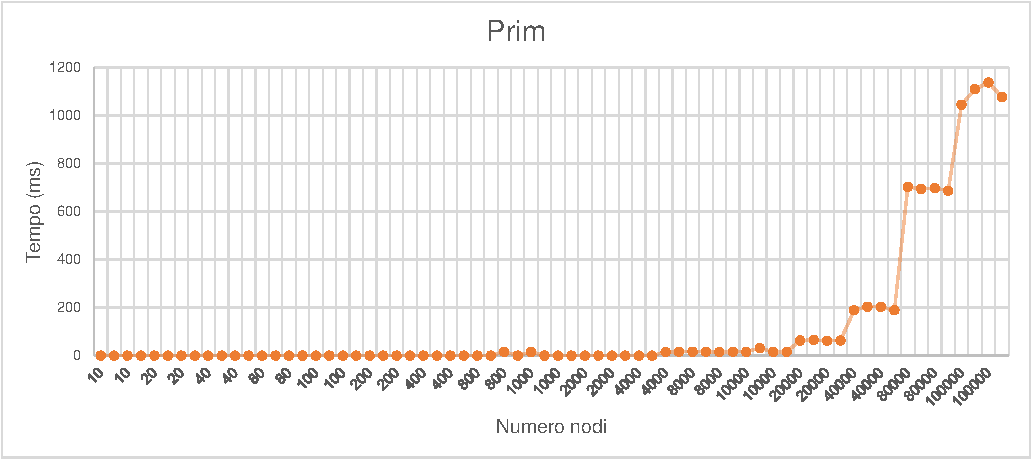
\includegraphics[scale=1]{grafici/prim.pdf}
\caption{Grafico andamento algoritmo di Prim}
\end{figure}

\begin{figure}[H]
\centering
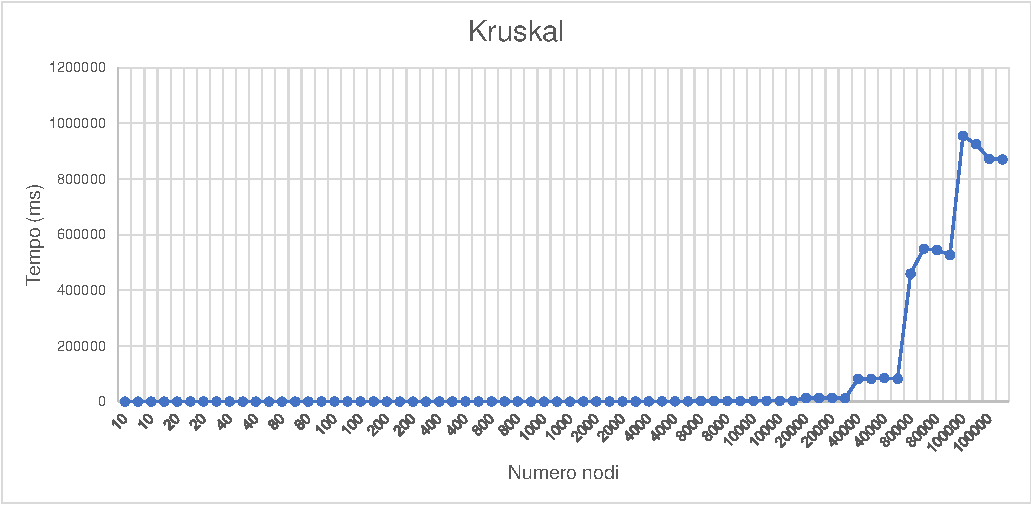
\includegraphics[scale=1]{grafici/kruskal.pdf}
\caption{Grafico andamento algoritmo di Kruskal}
\end{figure}

\begin{figure}[H]
\centering
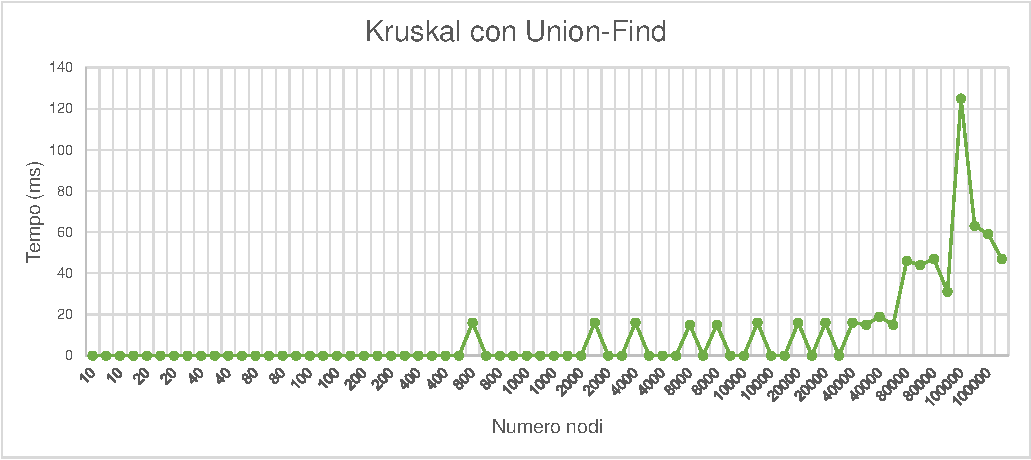
\includegraphics[scale=1]{grafici/kruskaluf.pdf}
\caption{Grafico andamento algoritmo di Kruskal con Union-Find}
\end{figure}

\begin{figure}[H]
\centering
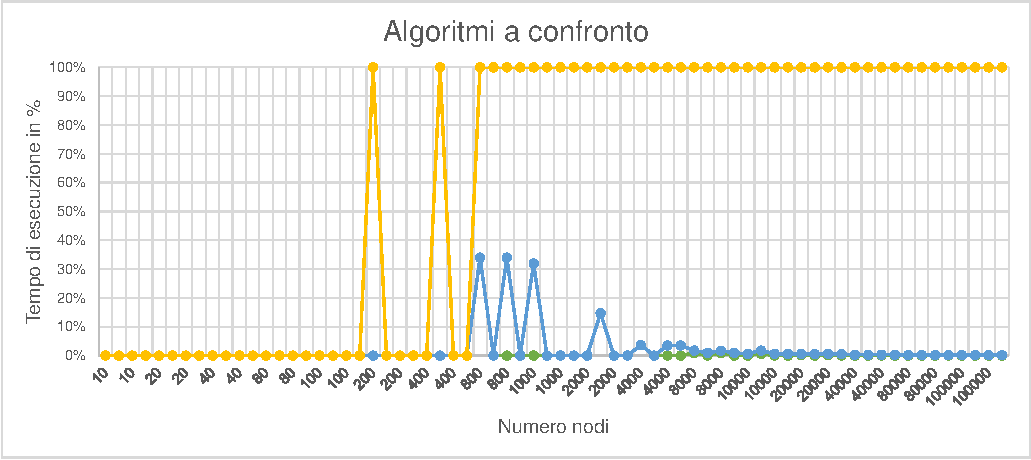
\includegraphics[scale=1]{grafici/confronto.pdf}
\caption{Grafico che mette in relazione i tempi di esecuzione dei tre algoritmi in base al tempo richiesto per la loro esecuzione}
\end{figure}

\section{Kruskal}
\begin{multicols}{2}
	\begin{table}[H]
		\centering
		\csvreader[head to column names,tabular=|l|l|l|l|,filter expr={test{\ifnumless{\nodi}{8000}}},
			table head=\hline\bfseries \# & \bfseries Numero nodi & \bfseries Tempo (ms)& \bfseries MST\\\hline,
			table foot=\hline]{kruskal.csv}{}{%
			\csvifoddrow{\slshape\thecsvrow & \slshape\nodi & \slshape\tempo & \slshape\mst}%
			{\bfseries\thecsvrow & \bfseries\nodi & \bfseries\tempo & \bfseries\mst}}
	\end{table}
	\begin{table}[H]
		\centering
		\csvreader[head to column names,tabular=|l|l|l|l|,filter expr={test{\ifnumgreater{\nodi}{4000}}},
			table head=\hline\bfseries \# & \bfseries Numero nodi & \bfseries Tempo (ms)& \bfseries MST\\\hline,
			table foot=\hline]{kruskal.csv}{}{%
			\csvifoddrow{\slshape\the\numexpr44+\thecsvrow & \slshape\nodi & \slshape\tempo & \slshape\mst}%
			{\bfseries\the\numexpr44+\thecsvrow & \bfseries\nodi & \bfseries\tempo & \bfseries\mst}}
	\end{table}
	\begin{figure}[H]
		\centering
		\begin{tikzpicture}
			\begin{axis}[xlabel=Numero nodi, ylabel=Tempo (ms)]
				\addplot table [x=nodi, y=tempo, col sep=comma] {kruskal.csv};
			\end{axis}
		\end{tikzpicture}
	\end{figure}
\end{multicols}
\newpage
\section{Kruskal con Union-Find}
\begin{multicols}{2}
	\begin{table}[H]
		\centering
		\csvreader[head to column names,tabular=|l|l|l|l|,filter expr={test{\ifnumless{\nodi}{8000}}},
			table head=\hline\bfseries \# & \bfseries Numero nodi & \bfseries Tempo (ms)& \bfseries MST\\\hline,
			table foot=\hline]{kruskal.csv}{}{%
			\csvifoddrow{\slshape\thecsvrow & \slshape\nodi & \slshape\tempo & \slshape\mst}%
			{\bfseries\thecsvrow & \bfseries\nodi & \bfseries\tempo & \bfseries\mst}}
	\end{table}
	\begin{table}[H]
		\centering
		\csvreader[head to column names,tabular=|l|l|l|l|,filter expr={test{\ifnumgreater{\nodi}{4000}}},
			table head=\hline\bfseries \# & \bfseries Numero nodi & \bfseries Tempo (ms)& \bfseries MST\\\hline,
			table foot=\hline]{kruskaluf.csv}{}{%
			\csvifoddrow{\slshape\the\numexpr44+\thecsvrow & \slshape\nodi & \slshape\tempo & \slshape\mst}%
			{\bfseries\the\numexpr44+\thecsvrow & \bfseries\nodi & \bfseries\tempo & \bfseries\mst}}
	\end{table}
	\begin{figure}[H]
		\centering
		\begin{tikzpicture}
			\begin{axis}[xlabel=Numero nodi, ylabel=Tempo (ms)]
				\addplot table [x=nodi, y=tempo, col sep=comma] {kruskaluf.csv};
			\end{axis}
		\end{tikzpicture}
	\end{figure}
\end{multicols}
\begin{figure}[H]
	\centering
	\begin{tikzpicture}
		\begin{axis}
			\addplot[ybar,fill] table [x=nodi, y=tempo, col sep=comma] {prim.csv};
			\addplot[ybar, green, fill] table [x=nodi, y=tempo, col sep=comma] {kruskal.csv};
			\addplot[ybar, red, fill] table [x=nodi, y=tempo, col sep=comma] {kruskaluf.csv};
		\end{axis}
	\end{tikzpicture}
\end{figure}
\end{document}
